\documentclass[english,oribibl]{llncs}
\usepackage[T1]{fontenc}
\usepackage[latin1]{inputenc}
\pagestyle{empty}
\usepackage{babel}
\usepackage{times}
\usepackage{epsfig}

\newcommand{\putfig}[5]{
  \begin{figure}[htbp]
  {\centering\resizebox*{#2}{#3}{\includegraphics{fig/#1.pdf}} \par}	
  \caption{#5\label{#4}}
  \end{figure}
}

\begin{document}

\title{\textsc{Epos} and Myrinet: Effective Communication Support for Parallel Applications Running on Clusters of Commodity Workstations\thanks{This research has been partially supported by the Federal University of Santa Catarina, by CAPES Foundation grant no. BEX 1083/96-1 and by Deutsche Forschungsgemeinschaft grant no. SCHR 603/1-1.}}

\author{Ant�nio Augusto Fr�hlich\inst{1}
\and Gilles Pokam Tientcheu\inst{1}
\and Wolfgang Schr�der-Preikschat\inst{2}}

\institute{
  GMD FIRST\\
  Kekul�sra�e 7\\
  D-12489 Berlin, Germany\\
  \email{\{guto|pokam\}@first.gmd.de}\\
  \texttt{http://www.first.gmd.de/\homedir guto}
\and
  University of Magdeburg\\
  Universit�tsplatz 2\\
  D-39106 Magdeburg, Germany\\
  \email{wosch@cs.uni-magdeburg.de}\\
  \texttt{http://ivs.cs.uni-magdeburg.de/\homedir wosch}
}

\maketitle


\raisebox{10cm}[0cm][0cm]{\makebox[\textwidth][r]{\copyright ~Springer-Verlag}}


\begin{abstract}

This paper presents the \textsc{Epos} approach to deliver parallel applications a high performance communication system. \textsc{Epos} is not an operating system, but a collection of components that can be arranged together to yield a variety of run-time systems, including complete operating systems. This paper focuses on the communication subsystem of \textsc{Epos}, which is comprised by the \emph{network adapter} and \emph{communicator} scenario-independent system abstractions. Like other \textsc{Epos} abstractions, they are adapted to specific execution scenarios by means of scenario adapters and are exported to application programmers via inflated interfaces. The paper also covers the implementation of the \emph{network adapter} system abstraction for the Myrinet high-speed network. This implementation is based on a carefully designed communication pipeline and achieved unprecedented performance.

\end{abstract}


\section{Introduction}

Undoubtedly, one of the most critical points to support parallel applications in distributed memory systems is communication. The challenge of enhancing communication performance, especially in cluster of commodity workstations, has motivated numerous well succeeded initiatives. At the hardware side, high-speed network architectures and fast buses counts for low-latency, high-bandwidth inter-node communication.  At the software side, perhaps the most significant advance has been to move the operating system out of the communication pathway. In this context, several forms of active messages, asynchronous remote copy, distributed shared memory, and even optimized versions of the traditional send/receive paradigm, have been proposed. Combined, all these initiatives left the giga-bit-per-second, application-to-application bandwidth barrier behind~\cite{Prylli:1998}. 

Nevertheless, good communication performance is hard to obtain when dealing with anything but the test applications supplied by the communication package developers.  Real applications, not seldom, present disappointing performance. We believe many performance losses to have a common root: the attempt to deliver a generic, all-purpose solution. Most research projects on high performance communication are looking for ``the best'' solution for a given architecture. However, a definitive best solution, independently of how fine-tuned to the underlying architecture it is, does not exist, whereas parallel applications simply communicate in quite different ways. Aware of this, many communication packages claim to be ``minimal basis'', upon which application-oriented abstractions can (have to) be implemented. One more time, there cannot be a best minimal base for all possible communication strategies. This contradiction between generic and optimal is presented in details in~\cite{Preikschat:1994}, and serves as motivation for the project \textsc{Epos}.

In \textsc{Epos}~\cite{Froehlich:sbac:1999}, we intend to give each application its own run-time support system, specifically constructed to satisfy its requirements (and nothing but its requirements). \textsc{Epos} is not an operating system, but a collection of components that can be arranged together in a framework to yield a variety of run-time systems, including complete operating systems. Besides application-orientation, the project aims on high performance and scalability to support parallel computing on clusters of commodity workstations. The following sections describe \textsc{Epos} communication system design, its implementation, and its performance.


\section{Communication System Design}

\textsc{Epos} has been conceived following the guidelines of traditional object-oriented design. However, scalability and performance constrains impelled us to define some \textsc{Epos} specific design elements. These design elements will be described next in the realm of the communication system.


\subsection{Scenario-independent System Abstractions}

Granularity plays a decisive role in any component-based system, since the decision about how fine or coarse components should be have serious implications. A system made up of a large amount of fine components will certainly achieve better performance than one made up of a couple of coarse components, since less unneeded functionality incurs less overhead. Nevertheless, a large set of fine components is more complex to configure and maintain.
  
In \textsc{Epos}, visible components have their granularity defined by the smallest-yet-application-ready rule. That is, each component made available to application programmers implements an abstract data type that is plausible in the application's run-time system domain. Each of these visible components, called \emph{system abstractions}, may in turn be implemented by simpler, non application-ready components.

In any run-time system, there are several aspects that are orthogonal to abstractions. For instance, a set of abstractions made SMP safe will very likely show a common pattern of synchronization primitives. In this way, we propose \textsc{Epos} system abstractions to be implemented as independent from execution scenario aspects as possible. These adaptable, scenario-independent system abstractions can then be put together with the aid of a \emph{scenario adapter}. 

Communication is handled in \textsc{Epos} by two sets of system abstractions: \emph{network adapters} and \emph{communicators}. The first set regards the abstraction of the physical network as a logical device able to handle one of the following strategies: datagram, stream, active message, or asynchronous remote copy. The second set of system abstractions deals with communication end-points, such as links, ports, mailboxes, distributed shared memory segments and remote object invocations. Since system abstractions are to be independent from execution scenarios, aspects such as reliability, sharing, and access control do not take part in their realizations; they are ``decorations'' that can be added by scenario adapters.

For most of \textsc{Epos} system abstractions, architectural aspects are also seen as part of the execution scenario, however, network architectures vary drastically, and implementing unique portable abstractions would compromise performance.  As an example, consider the architectural differences between Myrinet and SCI: a portable active message abstraction would waste Myrinet resources, while a portable asynchronous remote copy would waste SCI resources. Therefore, realizations for the \emph{network adapter} system abstraction shall exist for several network architectures. Some abstractions that are not directly supported by the network will be emulated, because we believe that, if the application really needs (or wants) them, it is better to emulate them close to the hardware.


\subsection{Scenario Adapters}

\textsc{Epos} system abstractions are adapted to specific execution scenarios by means of \emph{scenario adapters}. Currently, \textsc{Epos} scenario adapters are classes that wrap system abstractions, so that invocations of their methods are enclosed by the \texttt{enter} and  \texttt{leave} pair of scenario primitives. These primitives are usually inlined, so that nested calls are not generated. Besides enforcing scenario specific semantics, scenario adapters can also be used to ``decorate'' system abstractions, i.e., to extend their state and behavior.  For instance, all abstractions in a scenario may be tagged with a capability to accomplish access control.

In general, aspects such as application/operating system boundary crossing, synchronization, remote object invocation, debugging and profiling can easily be modeled with the aid of scenario adapters, thus making system abstractions, even if not completely, independent from execution scenarios.

The approach of writing pieces of software that are independent from certain aspects and later adapting them to a given scenario is usually referred to as \emph{Aspect-Oriented Programming}~\cite{Kiczales:ecoop:1997}. We refrain from using this expression, however, because much of AOP regards the development of languages to describe aspects and tools to automatically adapt components (\emph{weavers}). If ever used in \textsc{Epos}, AOP will give means but not goals.


\subsection{Inflated Interfaces}

Another important decision in a component-based system is how to export the component repository to application programmers. Every system with a reasonable number of components is challenged to answer this question. Visual and feature-based selection tools are helpless if the number of components exceeds a certain limit ---depending on the user expertise about the system, in our case the parallel application programmer expertise on operating systems. Tools can make the selection process user-friendlier, but certainly do not solve the user doubt about which selections to make. Moreover, users can usually point out what they want, but not how it should be implemented. That is, it is perhaps straightforward for a programmer to choose a mailbox as a communication end-point of a datagram oriented network, but perhaps not to decide whether features like multiplexing and dynamic buffer management should be added to the system.
  
The approach of \textsc{Epos} to export the component (system abstraction) repository is to present the user a restricted set of components. The adoption of scenario adapters already hides many components, since instead of a set of scenario specific realizations of an abstraction, only one abstraction and one scenario adapter are exported.  Nevertheless, \textsc{Epos} goes further on hiding components during the system configuration process. Instead of exporting individual interfaces for each flavor of an abstraction, \textsc{Epos} exports all of its flavors with a single \emph{inflated interface}. For example, the datagram, stream, active message, and asynchronous remote copy \emph{network adapters} are exported by a single~\texttt{Network\_Adapter} inflated interface as depicted in figure \ref{fig:interface}. 

\putfig{network_adapter}{!}{65mm}{fig:interface}{The \texttt{Network\_Adapter} inflated interface and its partial realizations.}

An inflated interface is associated to the classes that realize it through the \emph{selective, partial realize} relationship. This relationship is partial because only part of the inflated interface is realized, and it is selective because only one of the realizations can be bound to the inflated interface at a time. Each selective realize relationship is tagged with a key, so that defining a value for this key selects a realization for the corresponding interface. The way this relationship is implemented enables \textsc{Epos} to be configured by editing a single key table, and makes conditional compilations and ``makefile'' customizations unnecessary.

The process of binding an inflated interface to one of its realizations can be automated if we are able to clearly distinguish one realization from another.  In \textsc{Epos}, we identify abstraction realizations by the signatures of their methods. In this way, an automatic tool can collect signatures from the application and select adequate realizations for the corresponding inflated interfaces. Nevertheless, if two realizations have the same set of signatures, they must be exported by different interfaces.

The combination of \emph{system abstractions}, \emph{scenario adapters} and \emph{inflated interfaces}, effectively reduces the number of decisions the user has to take, since the visual selection tool will present a very restricted number of components, of which most have been preconfigured by the automatic binding tool. Besides, they enable application programmers to express their expectations concerning the run-time system simply by writing down well-known system object invocations.


\section{Communication System Implementation for Myrinet}

\textsc{Epos} is coded in C++ and is currently being developed to run either as a native ix86 system, or at guest-level on Linux. The ix86-native system can be configured either to be embedded in the application, or as $\mu$-kernel. The Linux-guest system is implemented by a library and a kernel loadable module. Both versions support the Myrinet high-speed network. \textsc{Epos} communication system implementation is detailed next.


\subsection{Platform Overview}

\textsc{Epos} is currently being implemented for a PC cluster available at GMD-FIRST.  This cluster consists nowadays of a server and 16 work nodes, each with an AMD Athlon processor running at 550 MHz, 128 MB of memory on a 100 MHz bus, and a 32 bits/33 MHz PCI bus in which a Fast-Ethernet and a Myrinet network adapter are plugged. This platform and some performance figures have been introduced in~\cite{Froehlich:euromicro:1998}, however, it is important to recall some of its characteristics in order to justify implementation decisions.

The Myrinet network adapter present in each node of our cluster has a processor, namely a LANai 4.1, 1 MB of memory and three DMA engines, respectively for transferring data between main memory and the memory on the network adapter, to send data to the network, and to receive data from the network. These DMA controllers can operate in parallel and perform two memory accesses per processor cycle. The memory on the Myrinet adapter is used to store the LANai control program and as communication buffer as well; it is also mapped into the main processor's address space, thus enabling data transfers without DMA assistance (programmed I/O).

A simple message exchange can be accomplished by using programmed I/O or DMA to write the message into the memory on the Myrinet adapter, and then signaling to the control program, by writing a shared flag, that a message of a given size is available in a certain memory location. The control program can then generate a message header with routing information and configure the send DMA controller to push the message into the network. The receiver side can be accomplished in a similar way, just adding a signal to the main processor to notify that a message has arrived. This can be done either by a shared flag polled by the main processor or via interruptions.

If the memory management scheme adopted on the node uses logical address spaces that are not contiguously mapped into memory, additional steps have to be included in order to support DMA. \textsc{Epos} can be configured to support either a single task (the typical case for MPI applications running on single processor nodes) or several tasks per node. The ix86-native, single-task version does not need any additional step, since logical and physical address spaces do match. The multi-tasking and Linux-guest version, however, allocate a contiguous buffer, of which the physical address is known, and give programmers two alternatives: write messages directly into the allocated buffer; or have messages copied into it. 

Figure \ref{fig:pipeline} depicts a message exchange between two applications (including the additional copies). The data transfer rate for each stage has been obtained and is approximately the following: 140 MB/s for the copy stages 1 and 5; 130 MB/s for the host/Myrinet DMA stages 2 and 4; and 160 MB/s for the send and receive DMA stages 3.1 and 3.2. Therefore, the total data transfer rate is limited to 130 MB/s by the host/Myrinet DMA stages. 

\putfig{send}{!}{!}{fig:pipeline}{Steps involved in a message exchange.}


\subsection{Communication Pipeline}

In order to deliver applications a communication bandwidth close to the 130 MB/s hardware limit the software overhead must be reduced to an insignificant level. Fortunately, a careful implementation and several optimization can help to get close to this limit. To begin with, the DMA controllers in the Myrinet adapter are able to operate in parallel, so that stages 2 and 3.1 of figure \ref{fig:pipeline}, as well as stages 4 and 3.2, can be overlapped. However, these stages are not intrinsically synchronous, i.e., there is no guarantee that starting stage 3.1 just after starting stage 2 will preserve message integrity. Therefore, overlapping will only be possible for different messages or, what is more interesting, different pieces of a message. We took advantage of this architectural feature to implement a communication pipeline for \textsc{Epos}.

\textsc{Epos} communication pipeline for Myrinet has been designed considering the time messages of different sizes spend at each stage of figure \ref{fig:pipeline}. This time includes the overhead for the stage (per-packet cost) and its effective data transfer rate (per-byte cost). It is important to notice that the overhead includes synchronization operations and the waiting time for the next stage to become available. According to Myrinet documentation, the delay between stages 3.1 and 3.2 is of 0.5 $\mu$s per switch hop. As this latency is much smaller then any other in the pipeline, we will consider stages 3.1 and 3.2 to completely overlap each other, thus yielding a single pipeline stage 3. 

A message sent through the network is now split in small packets that move through the stages of the pipeline. In order to sustain a transfer rate close to the maximum, at least two requirements must be fulfilled: first, the number of packets must be at least equal to the depth of the pipeline (five in our case), and second, the packet length must be such as to minimize the total message transmission time. To determine the optimal packet length for the pipeline, we modeled it according to the following rules:

\begin{itemize}
\item As soon as a packet \(n\) leaves a pipeline stage \(i\), it enters the next stage \(i+1\);

\item A packet \(n\) enters stage \(i\) of the pipeline as soon as packet \(n-1\) leaves it. 
\end{itemize}

In this way, we can compute the optimal packet length \(P_{optimal}\) by looking for a maximum of the function \(T(L,P)\), which represents the time a message of size \(L\), split in packets of length \(P\), takes to move through the pipeline~\cite{Wang:sigmetrics:1998}. This function can be expressed as the sum of the time a packet spends on each of the pipeline stages. Using a linear cost model~\cite{Rumeur:1994}, the time spent by a packet \(n\) in a stage \(i\) can be expressed as: 

\begin{equation}
 T_{i}^{(n)}=\beta _{i}+P\tau _{i}
\label{equ:I}
\end{equation}

\noindent where \(\beta _{i}\) is the constant per-packet cost assigned to stage \(i\), \(P\) is the packet size, and \(\tau _{i}\) the inverse of stage \(i\) bandwidth.

Taking in consideration the characteristics of the platform described earlier, we can assume the cost of the copy stages 1 and 5 to be approximately the same, since they involve the same hardware resources, i.e., processor and memory.  For the same reason we can consider the cost of stage 2 to be approximately the same of stage 4. Therefore, \( \beta _{1}\cong \beta _{5} \) and \( \tau _{1}\cong \tau _{5} \), while \( \beta _{2}\cong \beta _{4} \) and \( \tau _{2}\cong \tau _{4} \).  Since the bandwidth of the Myrinet network (160 MB/s) is greater than that of main memory copy (140 MB/s), which in turn is greater than that of the host/Myrinet DMA (130 MB/s), we can write the following inequality:

\begin{equation}
\tau _{2}\cong \tau _{4}>\tau _{1}\cong \tau _{5}>\tau _{3}
\label{equ:III}
\end{equation}
  
From the inequality \ref{equ:III} above, we can deduce an upper bound for the delay experienced by a packet traveling through the stage 3 of the pipeline (inequalities \ref{equ:IVa} and \ref{equ:IVb}); and also the delay experienced by the last packet of the message at stage 4 (inequality \ref{equ:IVc})\footnote{The overhead of upstream pipeline stages has to be considered because there is no analytical way to determine a relation among them. Even measurements are not possible, since execution time is not predictable in our CPUs.}.

\begin{equation}
\beta _{1}+\beta _{2}+\beta _{3}+P\tau _{2}>\beta _{3}+P\tau _{3}
\label{equ:IVa}
\end{equation}

\begin{equation}
\beta _{1}+\beta _{2}+\beta _{3}+P\tau _{2}>\beta _{1}+P\tau _{1}
\label{equ:IVb}
\end{equation}

\begin{equation}
\beta _{1}+\beta _{2}+P\tau _{2}>\beta _{1}+P\tau _{1}
\label{equ:IVc}
\end{equation}

\noindent Assuming that the message size \( L \) is an integer multiple of \( P \), the function \( T(L,P) \) could be expressed as:

\begin{equation}
T(L,P)=\sum ^{2}_{k=1}T^{(1)}_{k}+\sum ^{\lceil \frac{L}{P}\rceil }_{i=1}T^{(i)}_{3}+\sum ^{5}_{j=4}T^{(\lceil \frac{L}{P}\rceil )}_{j}
\label{equ:V}
\end{equation}

\noindent From the inequalities above, and from the approximations suggested earlier, we can express \( T(L,P) \) as:

\begin{equation}
T(L,P)\cong 2(2\beta _{1}+\beta _{2})+2(\tau _{1}+\tau _{2})P+\lceil \frac{L}{P}\rceil (\beta _{1}+\beta _{2}+\beta _{3}+P\tau _{2})
\label{equ:VII}
\end{equation}

\noindent and the optimal packet size can be computed by solving the following equation:

\begin{equation}
\frac{dT(L,P)}{dP}=0 \Rightarrow P_{optimal}=\sqrt{\frac{L(\beta _{1}+\beta _{2}+\beta _{3})}{2(\tau _{1}+\tau 2)}}
\label{equ:VIII}
\end{equation}

By applying a linear regression approximation~\cite{Jain:1991} to each stage of the pipeline on the set of predictor variables, which has been obtained from the non-pipelined transfer of messages of various sizes, we computed the values for \(\beta\) and \(\tau\) to be approximately the ones given in table \ref{tab:costs}.

\begin{table}[htbp]
\caption{Computed values for the per-packet cost \protect\( \beta \protect \) and inverse bandwidth \protect\( \tau \protect \) of each pipeline stage.\label{tab:costs}}
{\centering \begin{tabular}{lcc}
\hline 
stage~~&\(\beta _{i}\)(in \(\mu s\))~~&\(\tau _{i}\)(in\(\frac{\mu s}{KB}\))\\
\hline 
1, 5& 3.0 & 5.9\\
2, 4 & 0.6 & 7.6\\
3 & 1.3 & 7.5\\
\hline 
\end{tabular}\par}
\end{table} 

As an example, the calculated optimal packet length for a 64 KB message is 3490 bytes. In practice, 4 KB packets are to be used. We solved equation \ref{equ:VIII} for several message lengths in order to determine the optimal packet length for ranges of message lengths. With this information in hand, we implemented an adaptive pipeline that automatically selects the appropriate packet length according to the message length, thus minimizing the message transfer latency.  

\subsection{Short Messages}

Although the pipeline described above has a very low intrinsic overhead, programming DMA controllers and synchronizing pipeline stages may demand more time than it is necessary to send a short message via programmed I/O. In order to optimize the transfer of short messages using programmed I/O, which usually has a mediocre performance on PCs, we instructed our processors to collect individual write transactions that would traverse the PCI bridge to form 32 bytes chunks. Each chunk is then transferred in a burst transaction. This feature is enabled by selecting a ``combine'' cache policy for the pages that map the memory on the Myrinet adapter into the address space of the process. For the current implementation, messages shorter than 256 bytes are transferred in this way.


\subsection{Performance Evaluation}

We evaluate the performance of \textsc{Epos} \emph{network adapter} system abstraction, by measuring the latency and the bandwidth experienced at the application level. A single-task, ix86-native and a Linux-guest version have been considered. The one-way tests have been executed in the platform previously described and consist of one node sending messages of different sizes to an adjacent node, i.e., one connected to the same Myrinet switch. The results are presented in figure \ref{fig:performance}, and, when compared to the 130 MB/s limit, give an efficiency rate of 85\% for 64 KB messages in the Linux-guest version and 92\% in the native version.

\begin{figure}[htbp]
{\centering
  \resizebox*{0.495\columnwidth}{!}{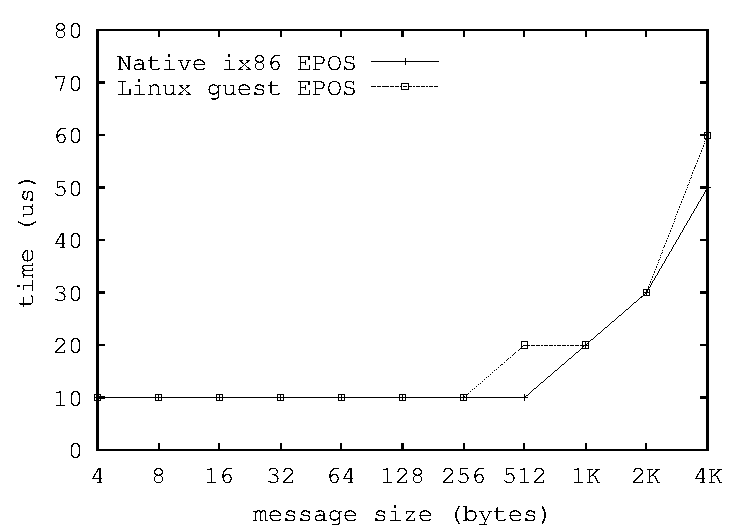
\includegraphics{gnu/latency.pdf}}
  \resizebox*{0.495\columnwidth}{!}{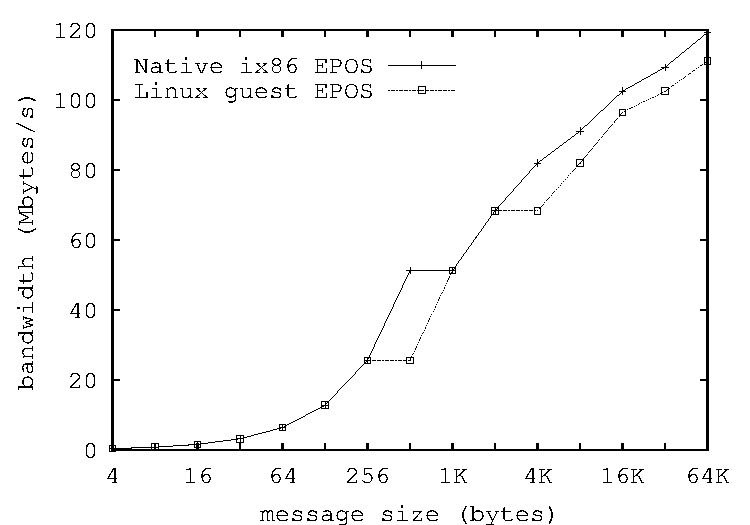
\includegraphics{gnu/bandwidth.pdf}}
  \par}
\caption{\textsc{Epos} \emph{network adapter} one-way latency (left) and bandwidth (right).\label{fig:performance}}
\end{figure}

\section{Conclusion}

In this paper we presented the \textsc{Epos} approach to deliver a high performance communication system to parallel applications running on clusters of commodity workstations. We demonstrated how \emph{system abstractions}, \emph{scenario adapters} and \emph{inflated interfaces} can simplify the process of run-time system configuration, mainly by reducing the number of decisions the user has to take. We also describe the \emph{network adapter} system abstraction implementation for the Myrinet high-speed network that interconnects the nodes in our PC cluster. 
 
The results obtained so far are highly positive and help to corroborate \textsc{Epos} design decisions. The evaluation of \textsc{Epos} \emph{network adapter} abstraction revealed performance figures that, as far as we are concerned, have no precedents in the Myrinet interconnected PC cluster history. However, \textsc{Epos} is a long term, open project that aims to deliver application-oriented run-time systems. Many system abstractions, scenario adapters, and tools are still to be implemented in order to support a considerable set of applications.

\bibliographystyle{plain}
\bibliography{hpcn2000}

\end{document}
